\documentclass[../TDTM3.tex]{subfiles}%

\begin{document}
\section[s]"2"{Méthode des vitesses initiales}
\enonce{%
	Le chlorure d'hydrogène (B) réagit sur le cyclohexène (A) avec formation de
	chlorocyclohexane (C), selon la réaction~:
	\[\ce{C6H10 + HCl \longrightarrow C6H11Cl}
		\quad
		\text{schématisée par}
		\quad
		\ce{A} + \ce{B} \longrightarrow \ce{C}
	\]
	On réalise une série d'expériences à \SI{25}{\degreeCelsius}, où l'on mesure la
	vitesse initiale $v_0$ de la réaction en fonction des concentrations molaires
	initiales $[\ce{A}]_0$ en cyclohexène et $[\ce{B}]_0$ en chlorure d'hydrogène
	dans le milieu réactionnel. Le volume du mélange est constant et égal à
	\SI{1}{L}. Les résultats sont rassemblés dans le tableau ci-dessous~:
	\begin{center}
		\begin{tabular}{lcccc}
			\toprule
			Expérience                       &
			1                                & 2           & 3           & 4           \\
			\midrule
			$[\ce{A}]_0$ ($\si{mol.L^{-1}}$) &
			\num{0.470}                      & \num{0.470} & \num{0.470} & \num{0.313} \\
			$[\ce{B}]_0$ ($\si{mol.L^{-1}}$) &
			\num{0.235}                      & \num{0.328} & \num{0.448} & \num{0.448} \\
			$v_0$ ($\SI{e-9}{mol.s^{-1}}$)   &
			\num{15.7}                       & \num{30.6}  & \num{57.1}  & \num{38.0}  \\
			\bottomrule
		\end{tabular}
	\end{center}
}

\QR{%
On désigne par $p$ et $q$ les ordres partiels initiaux de la réaction
par rapport au cyclohexène (A) et au chlorure d'hydrogène (B). Exprimer
la loi de vitesse initiale de cette réaction en fonction de $p$ et $q$.
}{%
Par définition,
\[ v_0 = k[\ce{A}]_0{}^p[\ce{B}]_0{}^q\]
}

\QR{%
	Déterminer $p$.
}{%
	Comme dans l'exercice~\ref{sec:mtdiff}, il suffit de trouver deux expériences où
	$[\ce{B}]_0$ est constante pour voir comment $v_0$ varie par
	multiplication de $[\ce{A}]_0$. Ici, dans les expériences 3 et 4,
	$[\ce{B}]_0 = \SI{0.448}{mol.L^{-1}}$. On a donc
	\begin{gather*}
		\left\{
		\begin{array}{rcl}
			v_{0,3} & = & k[\ce{B}]_0{}^q\times [\ce{A}]_{0,3}{}^p \\
			v_{0,4} & = & k[\ce{B}]_0{}^q\times [\ce{A}]_{0,4}{}^p
		\end{array}
		\right.
		\Leftrightarrow
		\frac{v_{0,3}}{v_{0,4}} = \left(
		\frac{[\ce{A}]_{0,3}}{[\ce{A}]_{0,4}}\right)^p\\
		\Leftrightarrow
		\boxed{
			p = \frac{\ln(v_{0,3}/v_{0,4})}{\ln([\ce{A}]_{0,3}/[\ce{A}]_{0,4})}
		}\\
		\mathrm{A.N.~:}\quad
		\boxed{p \approx 1}
	\end{gather*}
	On en conclut que \fbox{$p = 1$}, en supposant l'ordre entier.
}

\QR{%
	Déterminer $q$~; en déduire l'ordre global de la réaction.
}{%
	On fait de même avec les expériences 1 et 2 par exemple, où cette fois
	c'est $[\ce{A}]_0$ qui est constante. On trouve alors
	\begin{gather*}
		\boxed{
			q = \frac{\ln(v_{0,1}/v_{0,2})}{\ln([\ce{B}]_{0,1}/[\ce{B}]_{0,2})}
		}\\
		\mathrm{A.N.~:}\quad
		\boxed{q \approx 2}
	\end{gather*}
	On en conclut que \fbox{$q = 2$}, en supposant l'ordre entier. L'ordre
	global, défini par $p+q$, est donc \fbox{$p+q = 3$}.
}
\QR{%
Calculer la constante cinétique de la réaction.
}{%
Pour plus de précision, on peut tracer une régression linéaire de $v_0
	= f([\ce{A}]_0[\ce{B}]_0{}^2)$ avec
\[y = ax
	\qavec
	\left\{
	\begin{array}{rcl}
		y & = & v_0                      \\
		a & = & k                        \\
		x & = & [\ce{A}]_0[\ce{B}]_0{}^2
	\end{array}
	\right.
\]
\begin{minipage}{0.45\linewidth}
	On trouve bien ici une droite avec un coefficient de corrélation
	$r^2 = \num{0.99997}$, confirmant que l'\textbf{ordre global} est
	compatible avec 3. Le coefficient directeur donne directement $k$,
	et on a
	\[\boxed{k = \SI{6.05e-7}{mol^{-2}.L^2.s^{-1}}}\]
\end{minipage}
\hfill
\begin{minipage}{0.45\linewidth}
	\begin{center}
		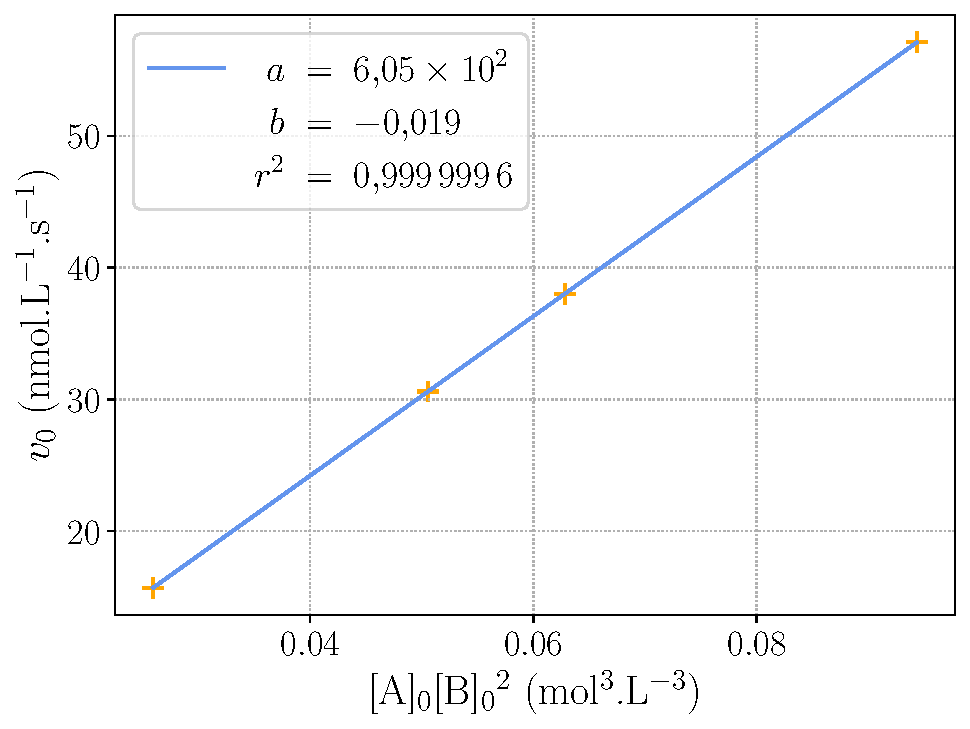
\includegraphics[width=\linewidth]{exo5_k}
	\end{center}
\end{minipage}
}
\QR{%
Dans le cas d'un mélange stœchiométrique en A et B, déterminer la loi
de vitesse de la réaction en fonction de $[\ce{A}]$. En déduire l'équation
différentielle satisfaite par $[\ce{A}](t)$, puis la résoudre.
}{%
Si le mélange est stœchiométrique, cela veut dire que les concentrations des
réactifs sont égaux à chaque instant, soit $[\ce{A}] = [\ce{B}]$. Ainsi, la loi
de vitesse serait
\begin{DispWithArrows*}
	\Aboxed{v = k [\ce{A}]^3
		&=
		- \dv{[\ce{A}]}{t}}
	\CArrow{$\times (-1)$}
	\\\Lra
	\dv{[\ce{A}]}{t}
	&=
	- k[\ce{A}](t)^3
	\Arrow{Séparation et $\DS \int$}
	\\\Lra
	\int_{[\ce{A}]_0}^{[\ce{A}](t)} \frac{\dd{[\ce{A}]}}{[\ce{A}](t)^3}
	&=
	-k \int_{t=0}^{t} \dt
	\Arrow{$\left( [\ce{A}]^{-2} \right)' = -2 \frac{\dd{[\ce{A}]}}{[\ce{A}](t)^3}$}
	\\\Lra
	\int_{[\ce{A}]_0}^{[\ce{A}](t)} \dd{\left( -\frac{1}{2}[\ce{A}]^2 \right)}
	&=
	-k \int_{t=0}^{t} \dt
	\Arrow{On intègre}
	\\\Lra
	-\frac{1}{2} \left( \frac{1}{[\ce{A}](t)^2} - \frac{1}{[\ce{A}]_0{}^2} \right)
	&=
	-k (t-0)
	\CArrow{$\times (-2)$}
	\\\Lra
	\Aboxed{%
	\frac{1}{[\ce{A}](t)^2} &= 2kt + \frac{1}{[\ce{A}]_0{}^2}
	}
\end{DispWithArrows*}
}
\end{document}
